\documentclass[../main.tex]{subfiles}

\begin{document}

\section{Factor de estructura}

\subsection{Graficas enteriores}

En la siguiente gráfica no me hace sentido los picos del factor de estructura.

\begin{figure}[ht!]
    \centering
    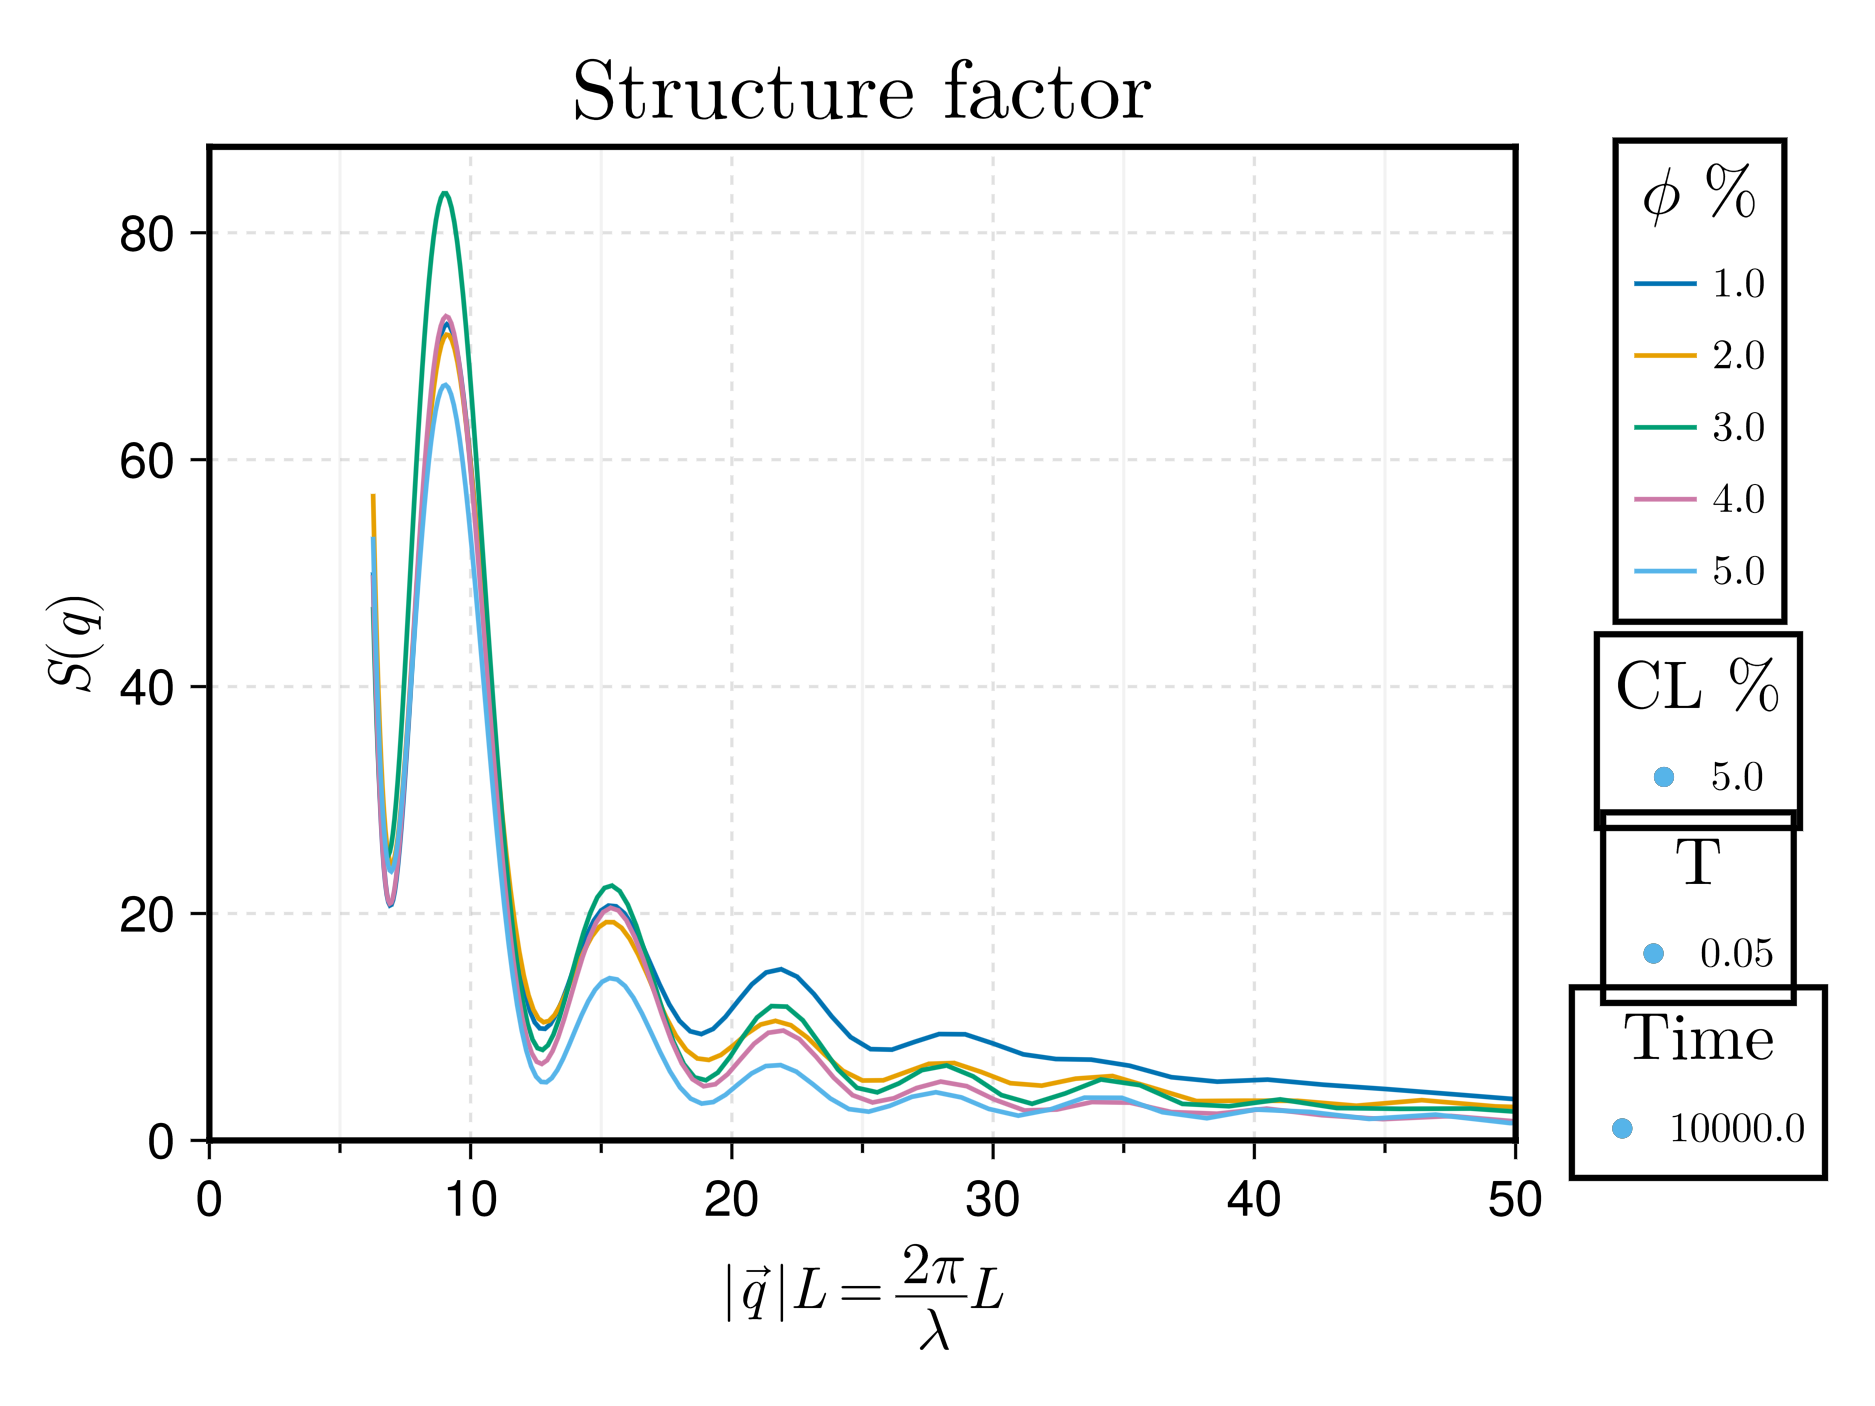
\includegraphics[width=0.9\textwidth]{../Figures/may4/fig_StructureFactor_tf_xL.png}
    \caption{Comparación de los factores de estructura en el tiempo final de la simulación para distintas concentraciones.}
\end{figure}

En la siguiente gráfica se muestra la evolución temporal del factor de estructura de una sola concentración.

\begin{figure}[ht!]
    \centering
    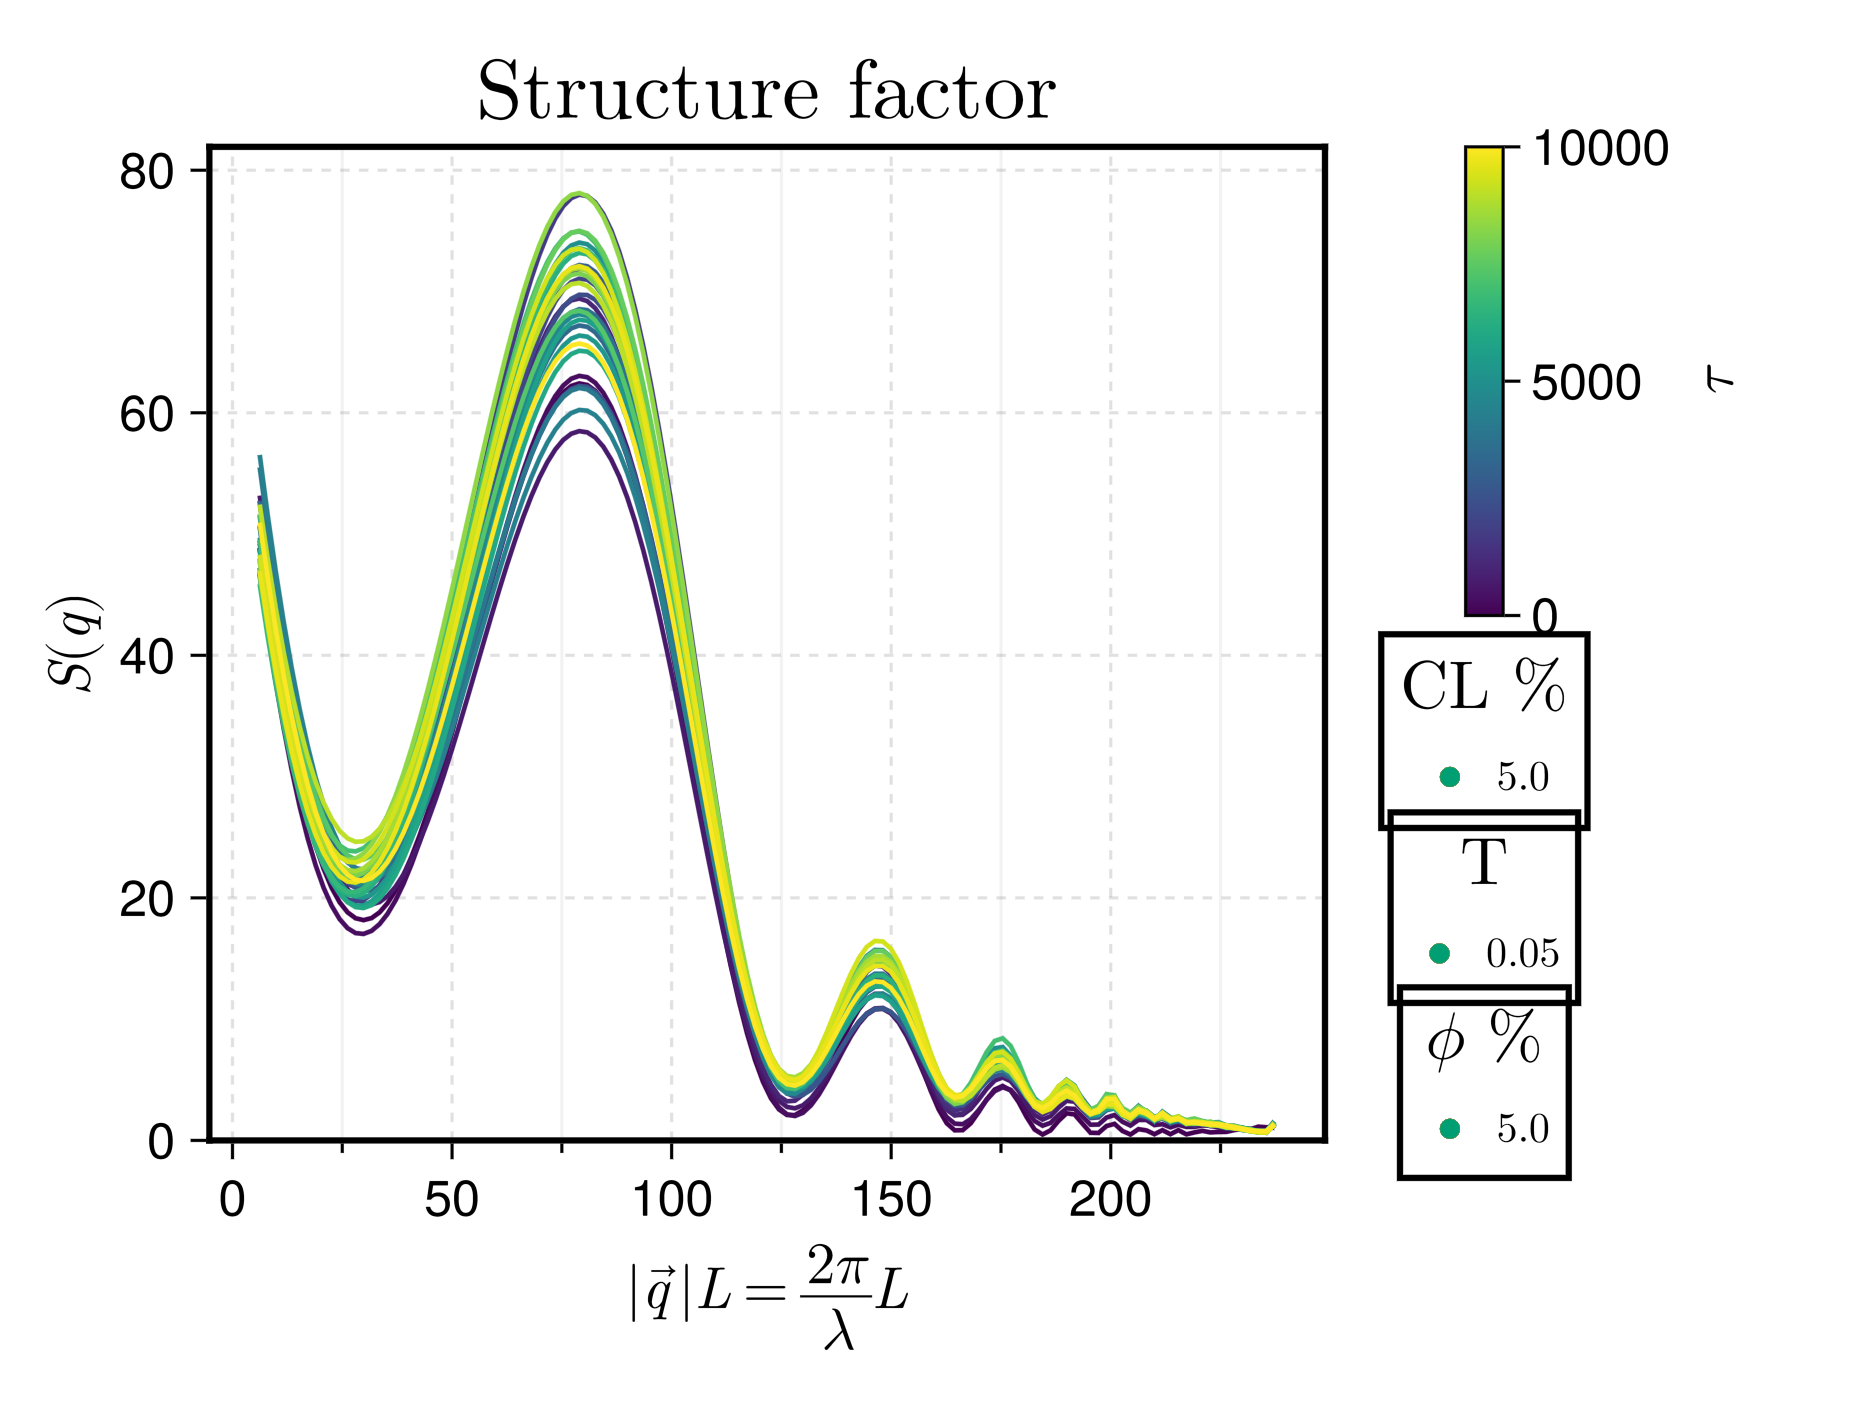
\includegraphics[width=0.9\textwidth]{../Figures/may4/structureFactor_timeSeries_phi5.png}
    \caption{Evolución temporal del factor de estructura para una sola fracción de empaquetamiento.}
\end{figure}

\subsection{Correcciones al código}

Pues tuve que corregir el código para calcular el factor de estructura.
Esto fueron los siguientes errores:
\begin{itemize}
    \item El dominio de la magnitud del vactor de onda no estaba bien definido
    \item los dominios espaciales para el producto punto no estaban equiespaciados
    \item La evaluación del producto solo se evaluaba parcialmente
    \item El promedio de las magnitudes estaba mal ejecutado
\end{itemize}

\subsection{Graficas después de los cambios}

\begin{figure}[ht!]
    \centering
    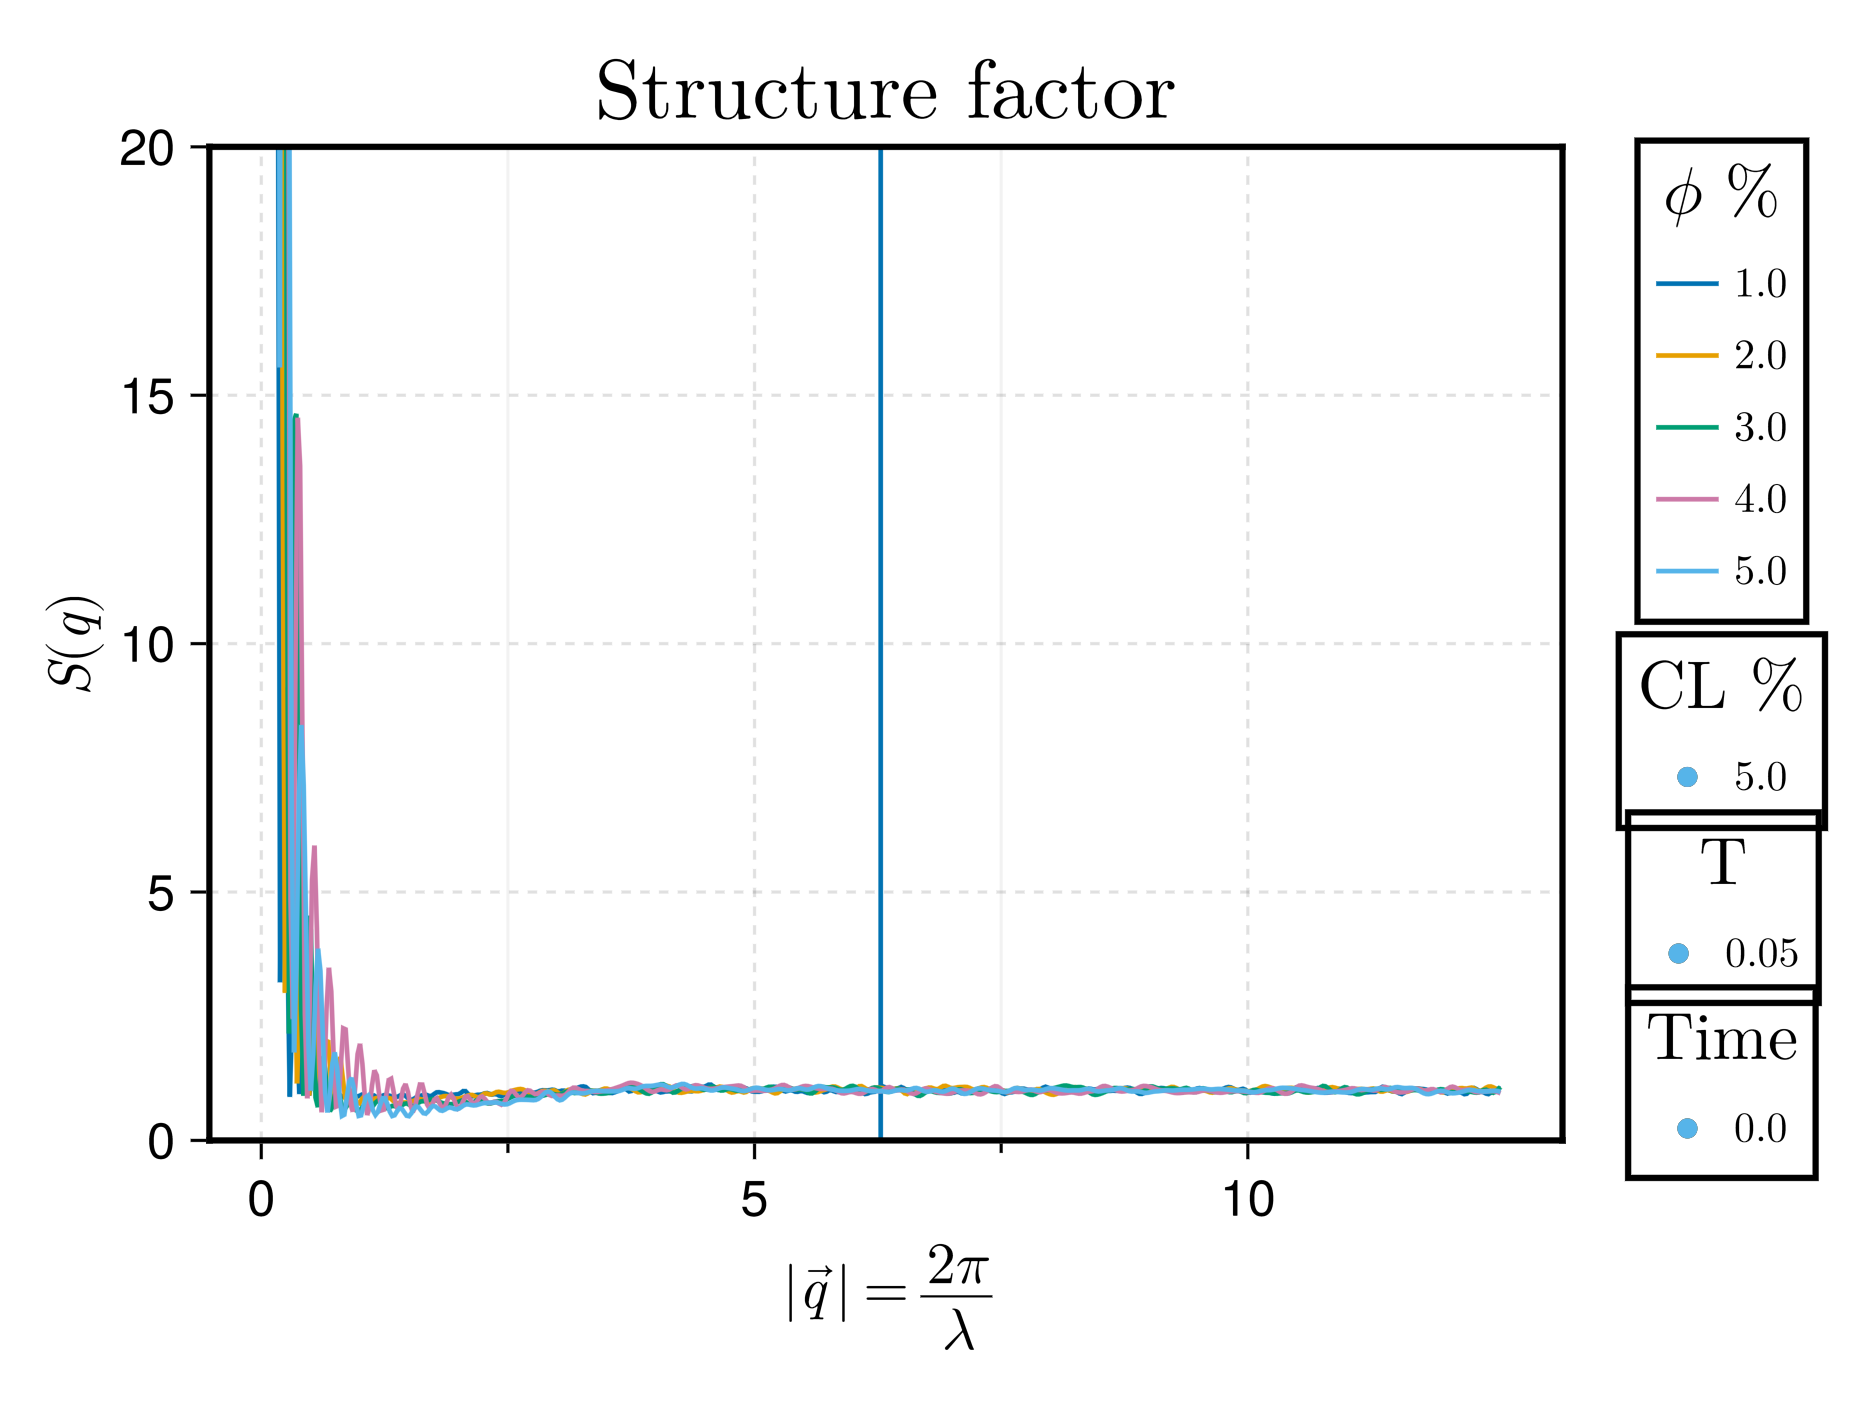
\includegraphics[width=0.9\textwidth]{../Figures/may4/fig_factorEstructuraCambios_to.png}
    \caption{Comparación de los factores de estructura en el tiempo inicial de la simulación para distintas concentraciones. La línea vertical está ubicada en: \(2\pi\).}
\end{figure}

\begin{figure}[ht!]
    \centering
    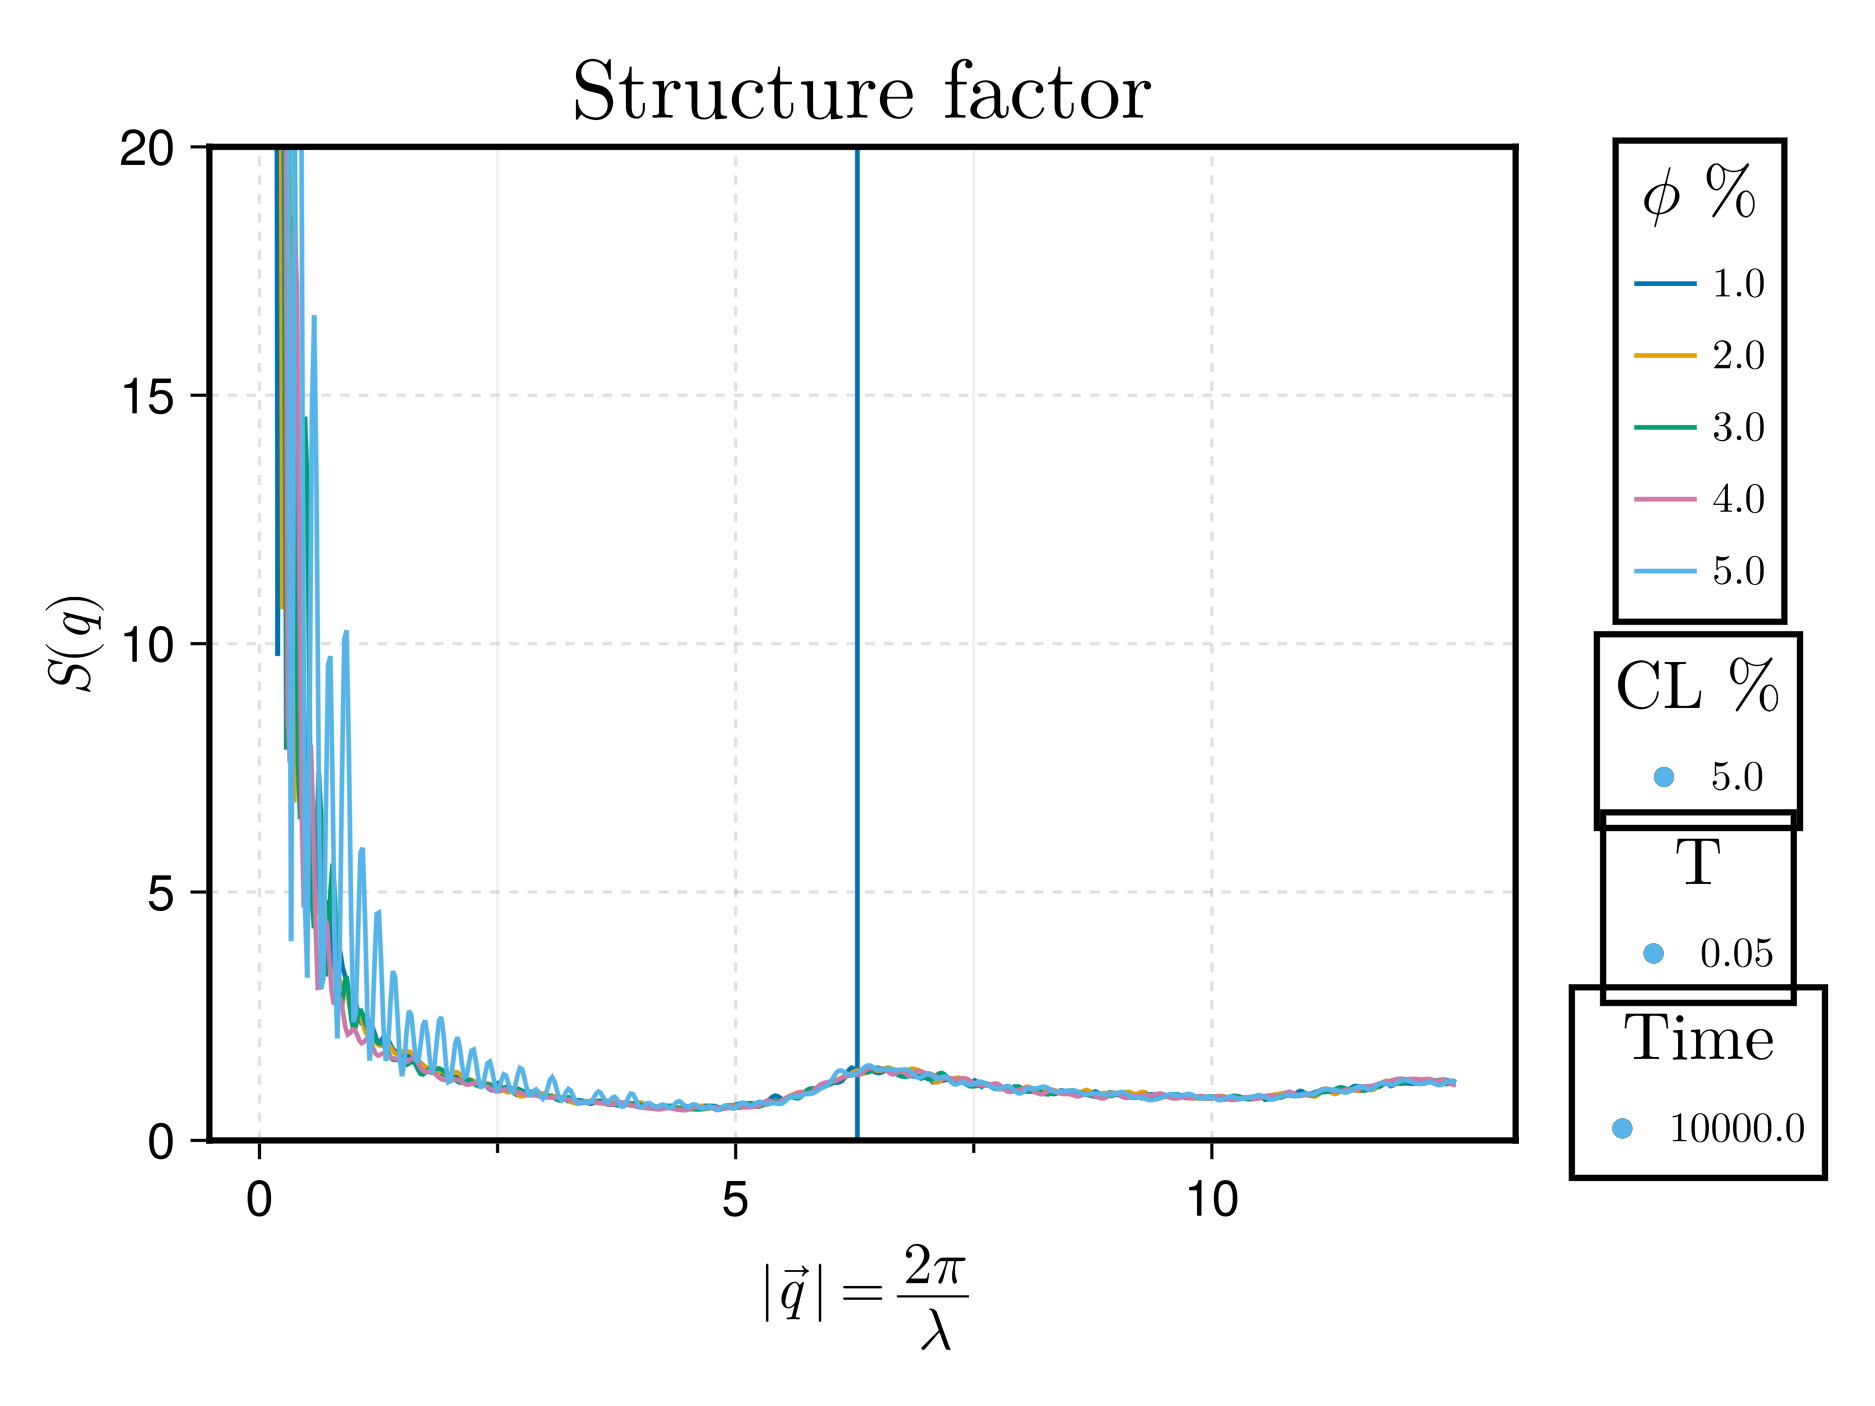
\includegraphics[width=0.9\textwidth]{../Figures/may4/fig_factorEstructuraCambios_tf.png}
    \caption{Comparación de los factores de estructura en el tiempo final de la simulación para distintas concentraciones. La línea vertical está ubicada en: \(2\pi\).}
\end{figure}

Las graficas anteriores solo muestran que hay un pico cuando \(\lambda=1\), es decir en el diámetro de las partículas centrales.
Estaba esperando un pico en \(\lambda=1.2\), porque esa es la distancia entre partículas centrales en las que se tiene el mínimo de potencial entre los patches.


Las siguientes gráficas solamente se escala el factor de estructura por la longitud de la caja.

\begin{figure}[ht!]
    \centering
    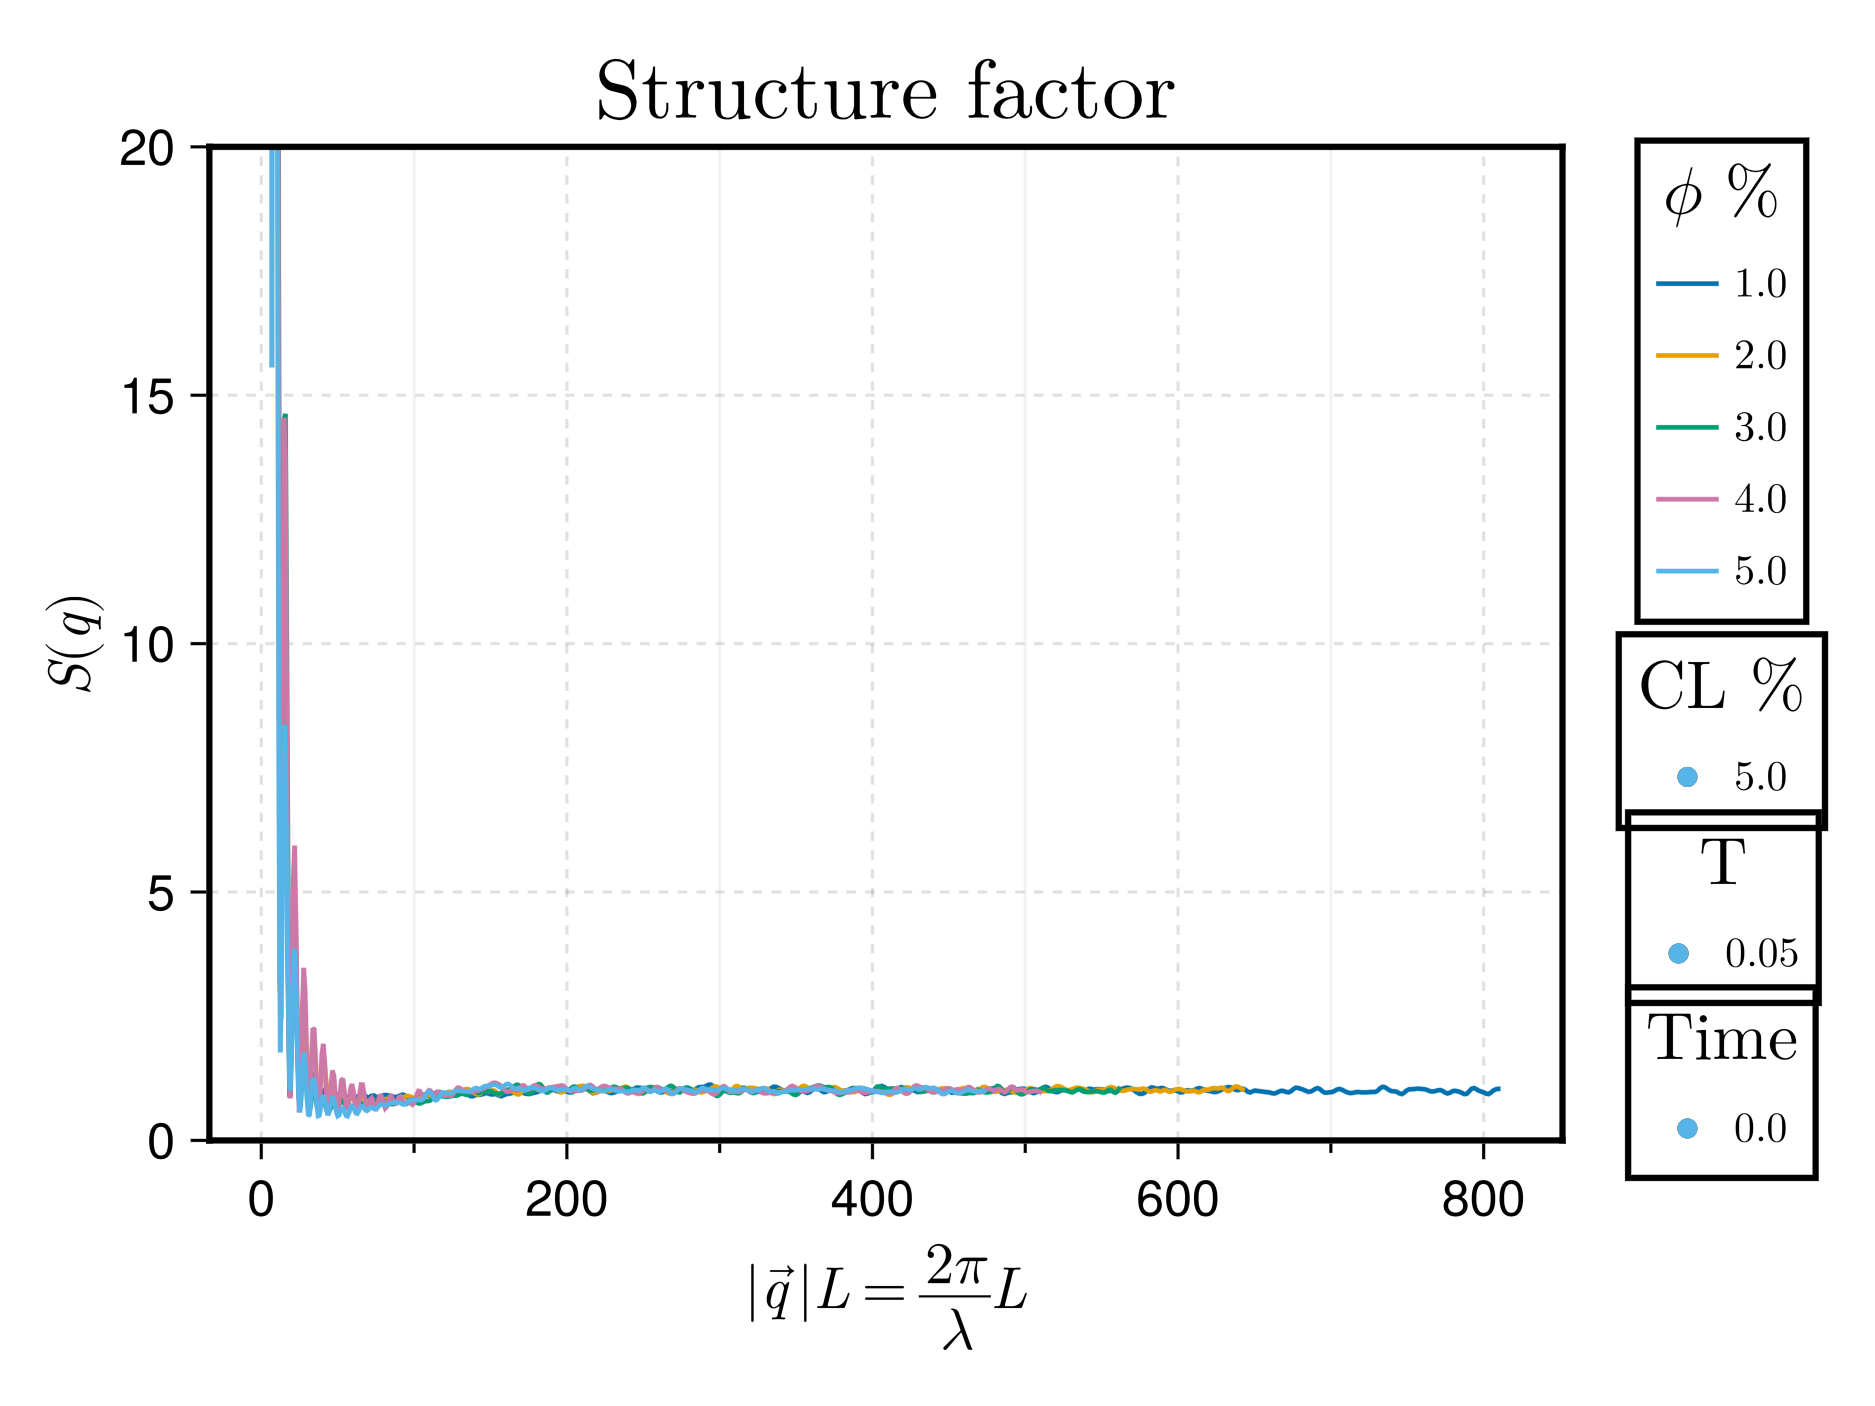
\includegraphics[width=0.9\textwidth]{../Figures/may4/fig_factorEstructuraCambios_to_xL.png}
    \caption{Comparación de los factores de estructura en el tiempo inicial de la simulación para distintas concentraciones. Las líneas verticales están ubicadas en: \(2\pi/1.2,\quad 2\pi/(2*1.2),\quad 2\pi/(3*1.2)\).}
\end{figure}

\begin{figure}[ht!]
    \centering
    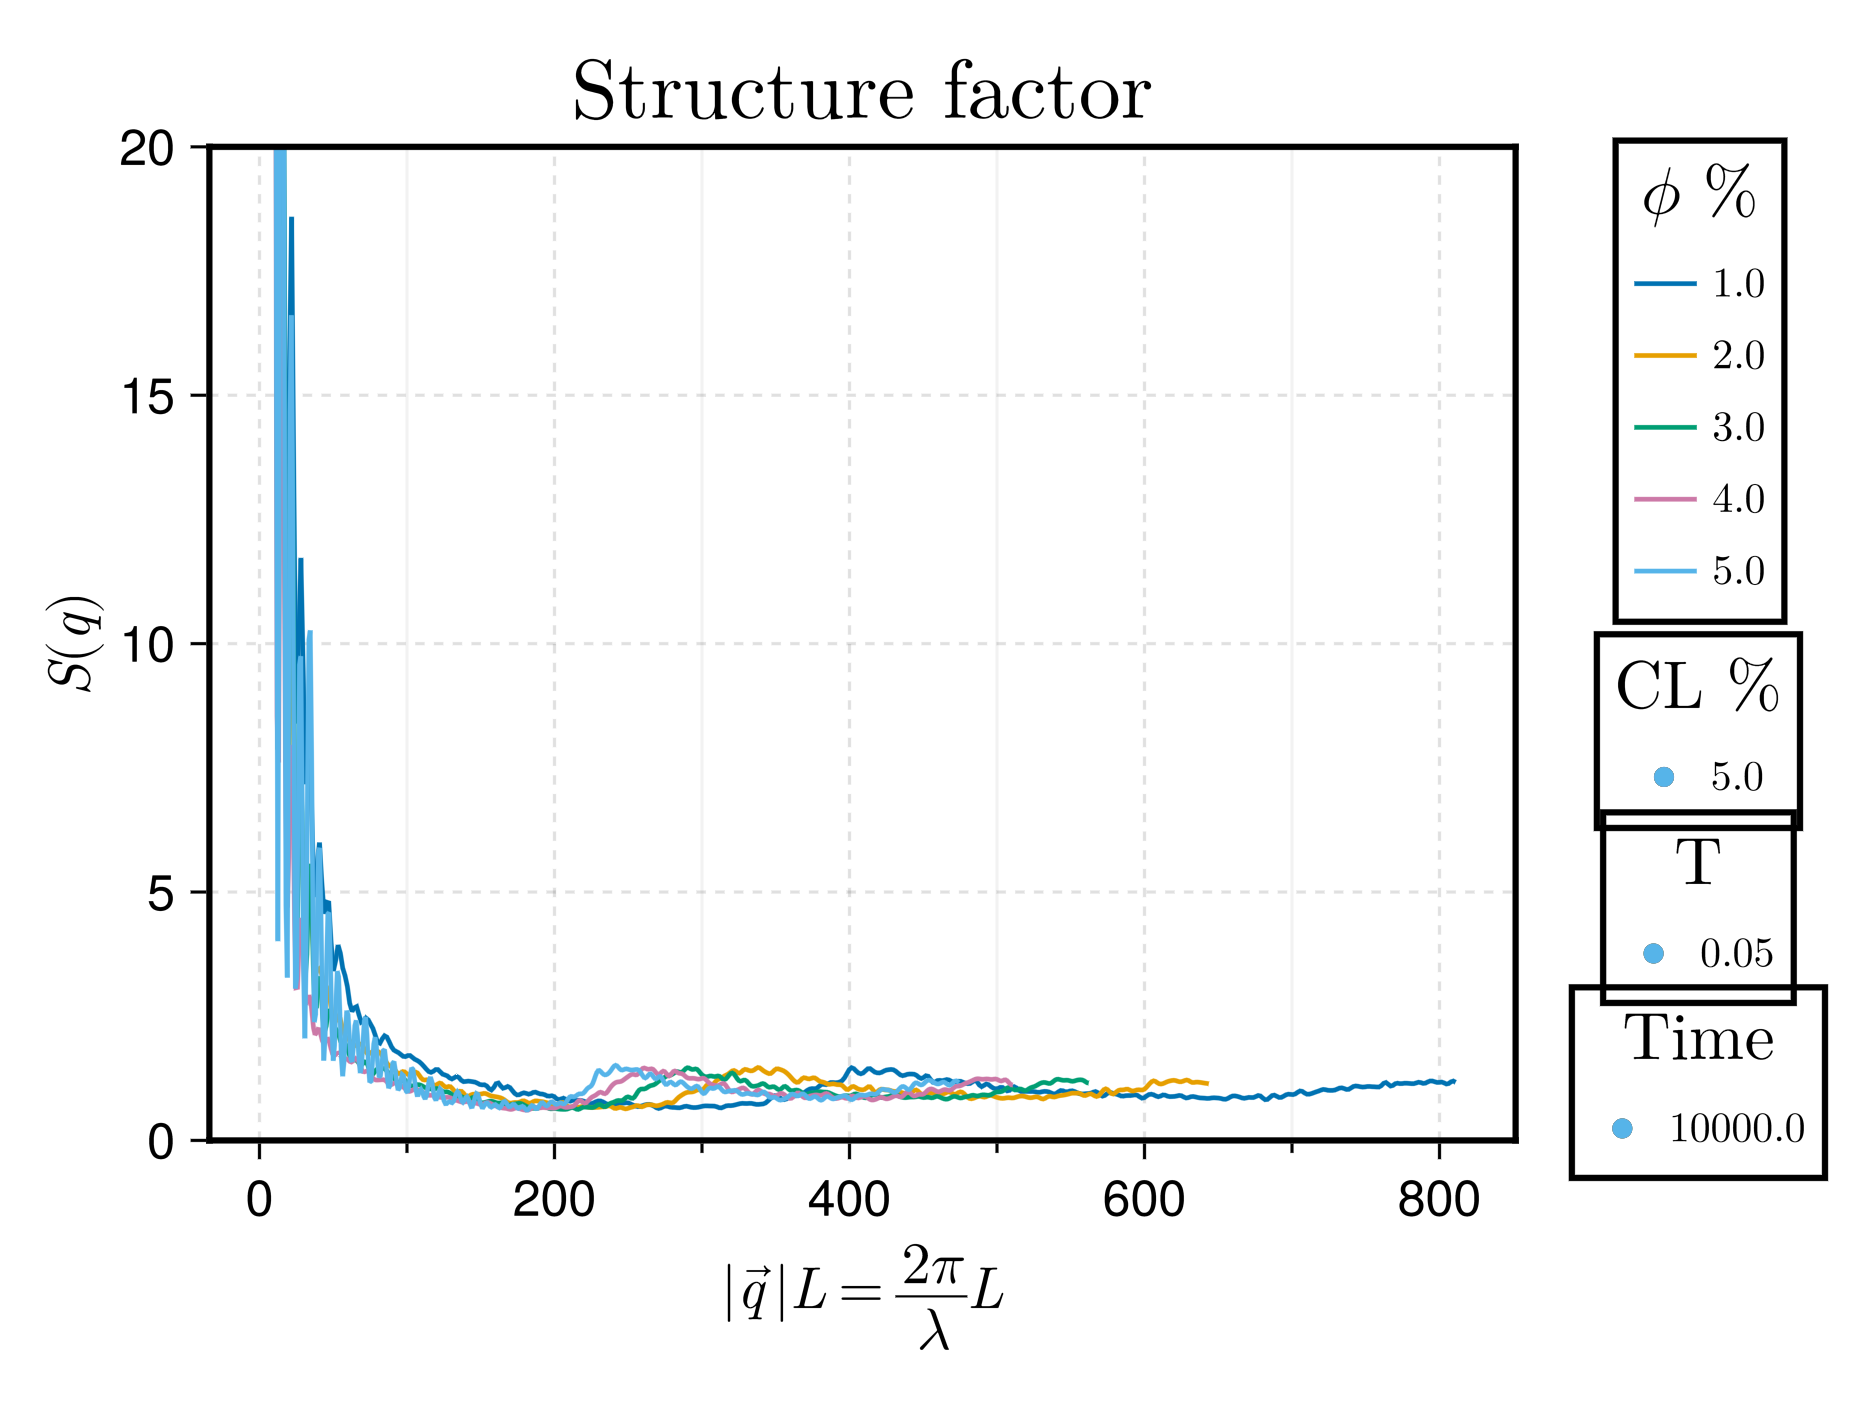
\includegraphics[width=0.9\textwidth]{../Figures/may4/fig_factorEstructuraCambios_tf_xL.png}
    \caption{Comparación de los factores de estructura en el tiempo final de la simulación para distintas concentraciones. Las líneas verticales están ubicadas en: \(2\pi/1.2,\quad 2\pi/(2*1.2),\quad 2\pi/(3*1.2)\).}
\end{figure}

No me hace sentido escalar el dominio del vector de onda en términos del tamaño de la caja.

\newpage

\section{Graficas con un domino más acotado}

Ahora se busca que \(\lambda\in[1,L]\), es decir que \(|\vec{q}|\in[2\pi/L,2\pi]\).

\begin{figure}[ht!]
    \centering
    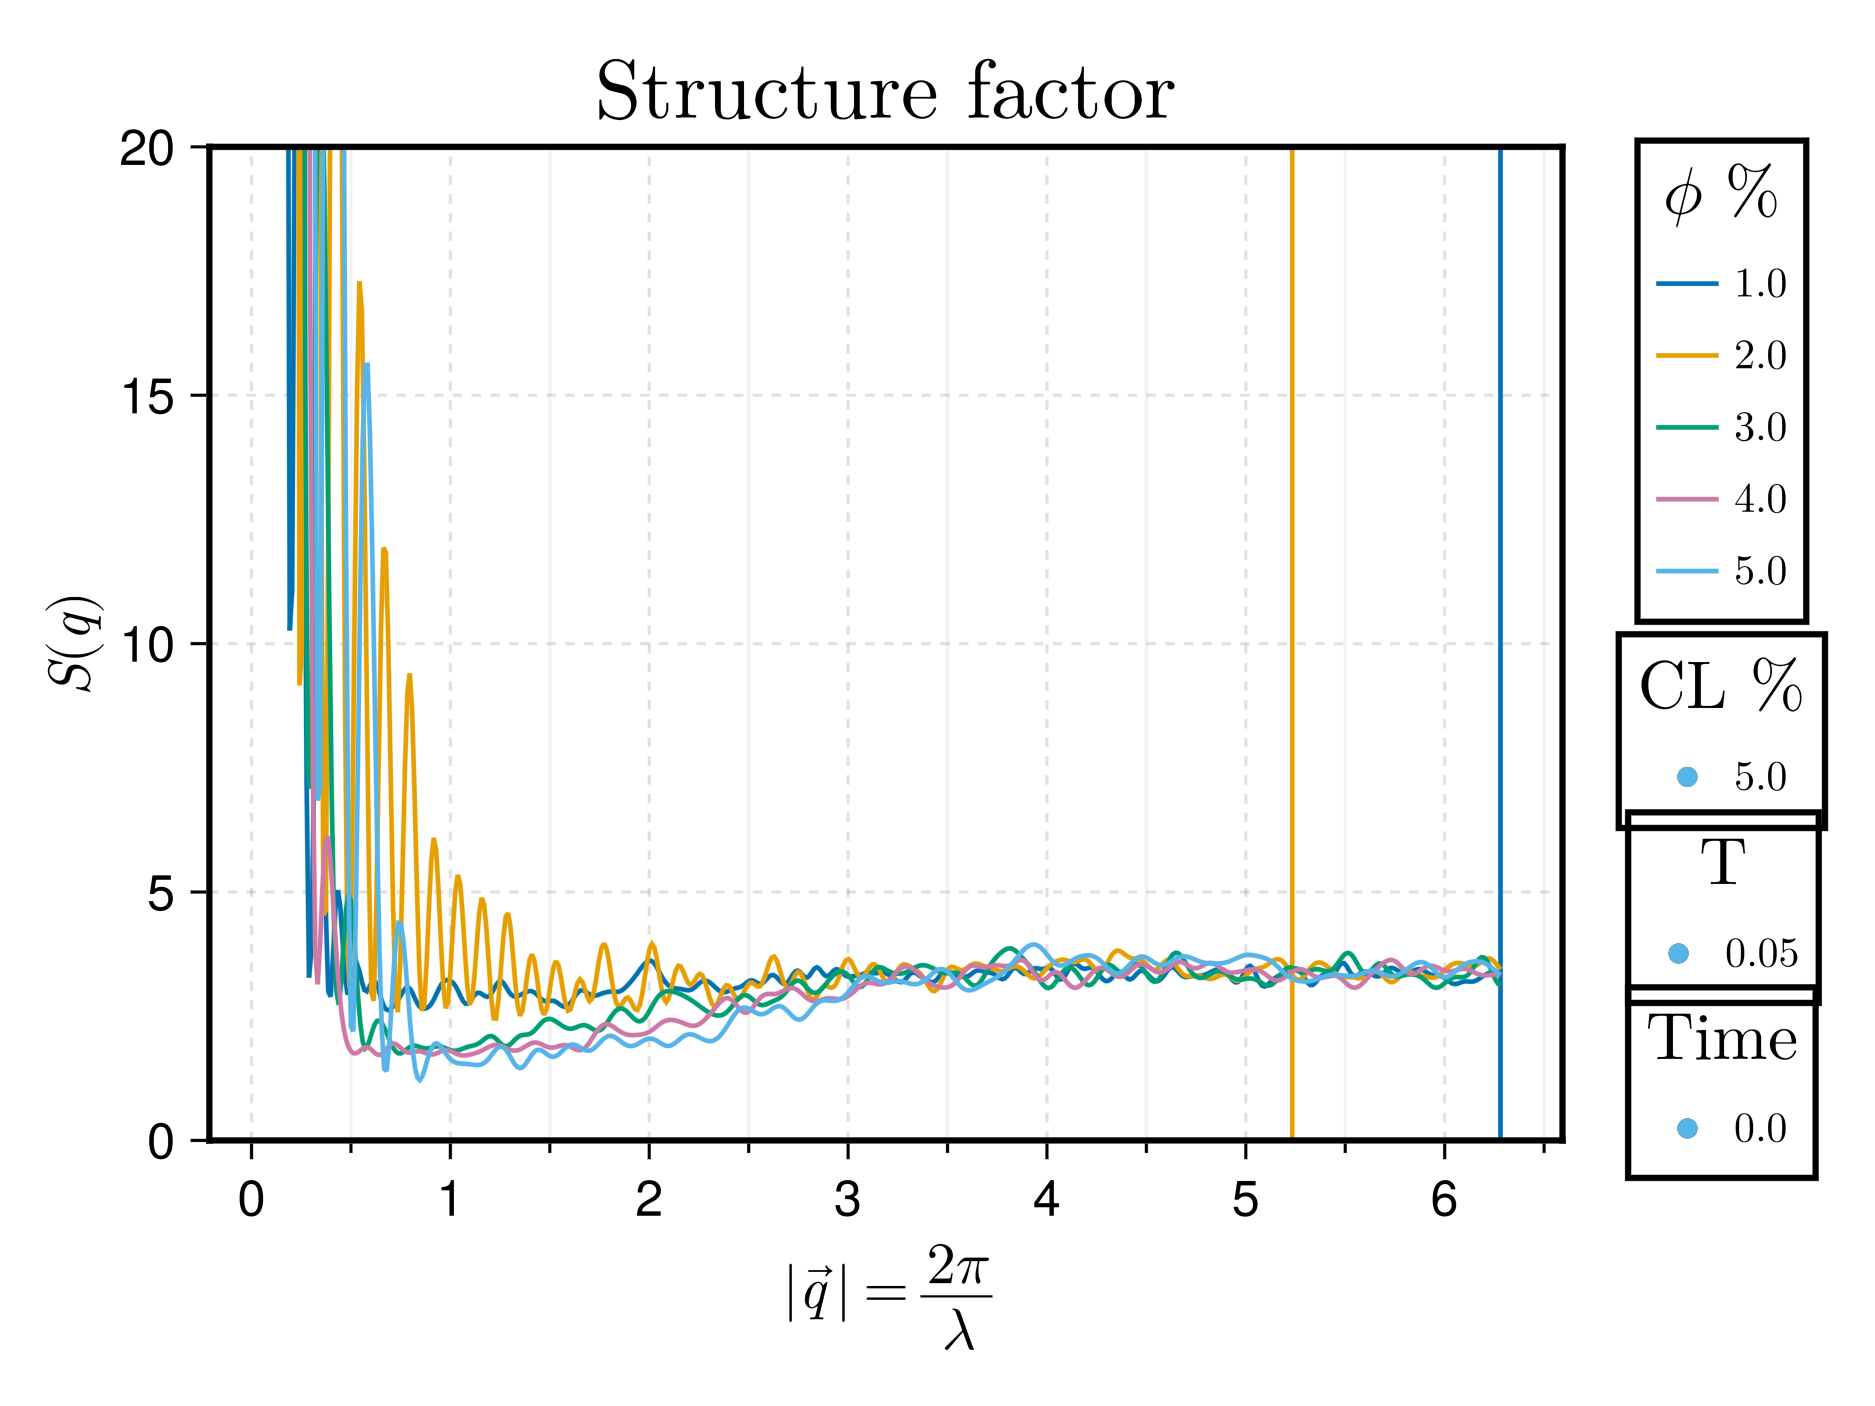
\includegraphics[width=0.9\textwidth]{../Figures/may4/fig_factorEstructuraCambios_to_zoom.png}
    \caption{Comparación de los factores de estructura en el tiempo inicial de la simulación para distintas concentraciones. La línea vertical está ubicada en: \(2\pi,2\pi/1.2\).}
\end{figure}

\begin{figure}[ht!]
    \centering
    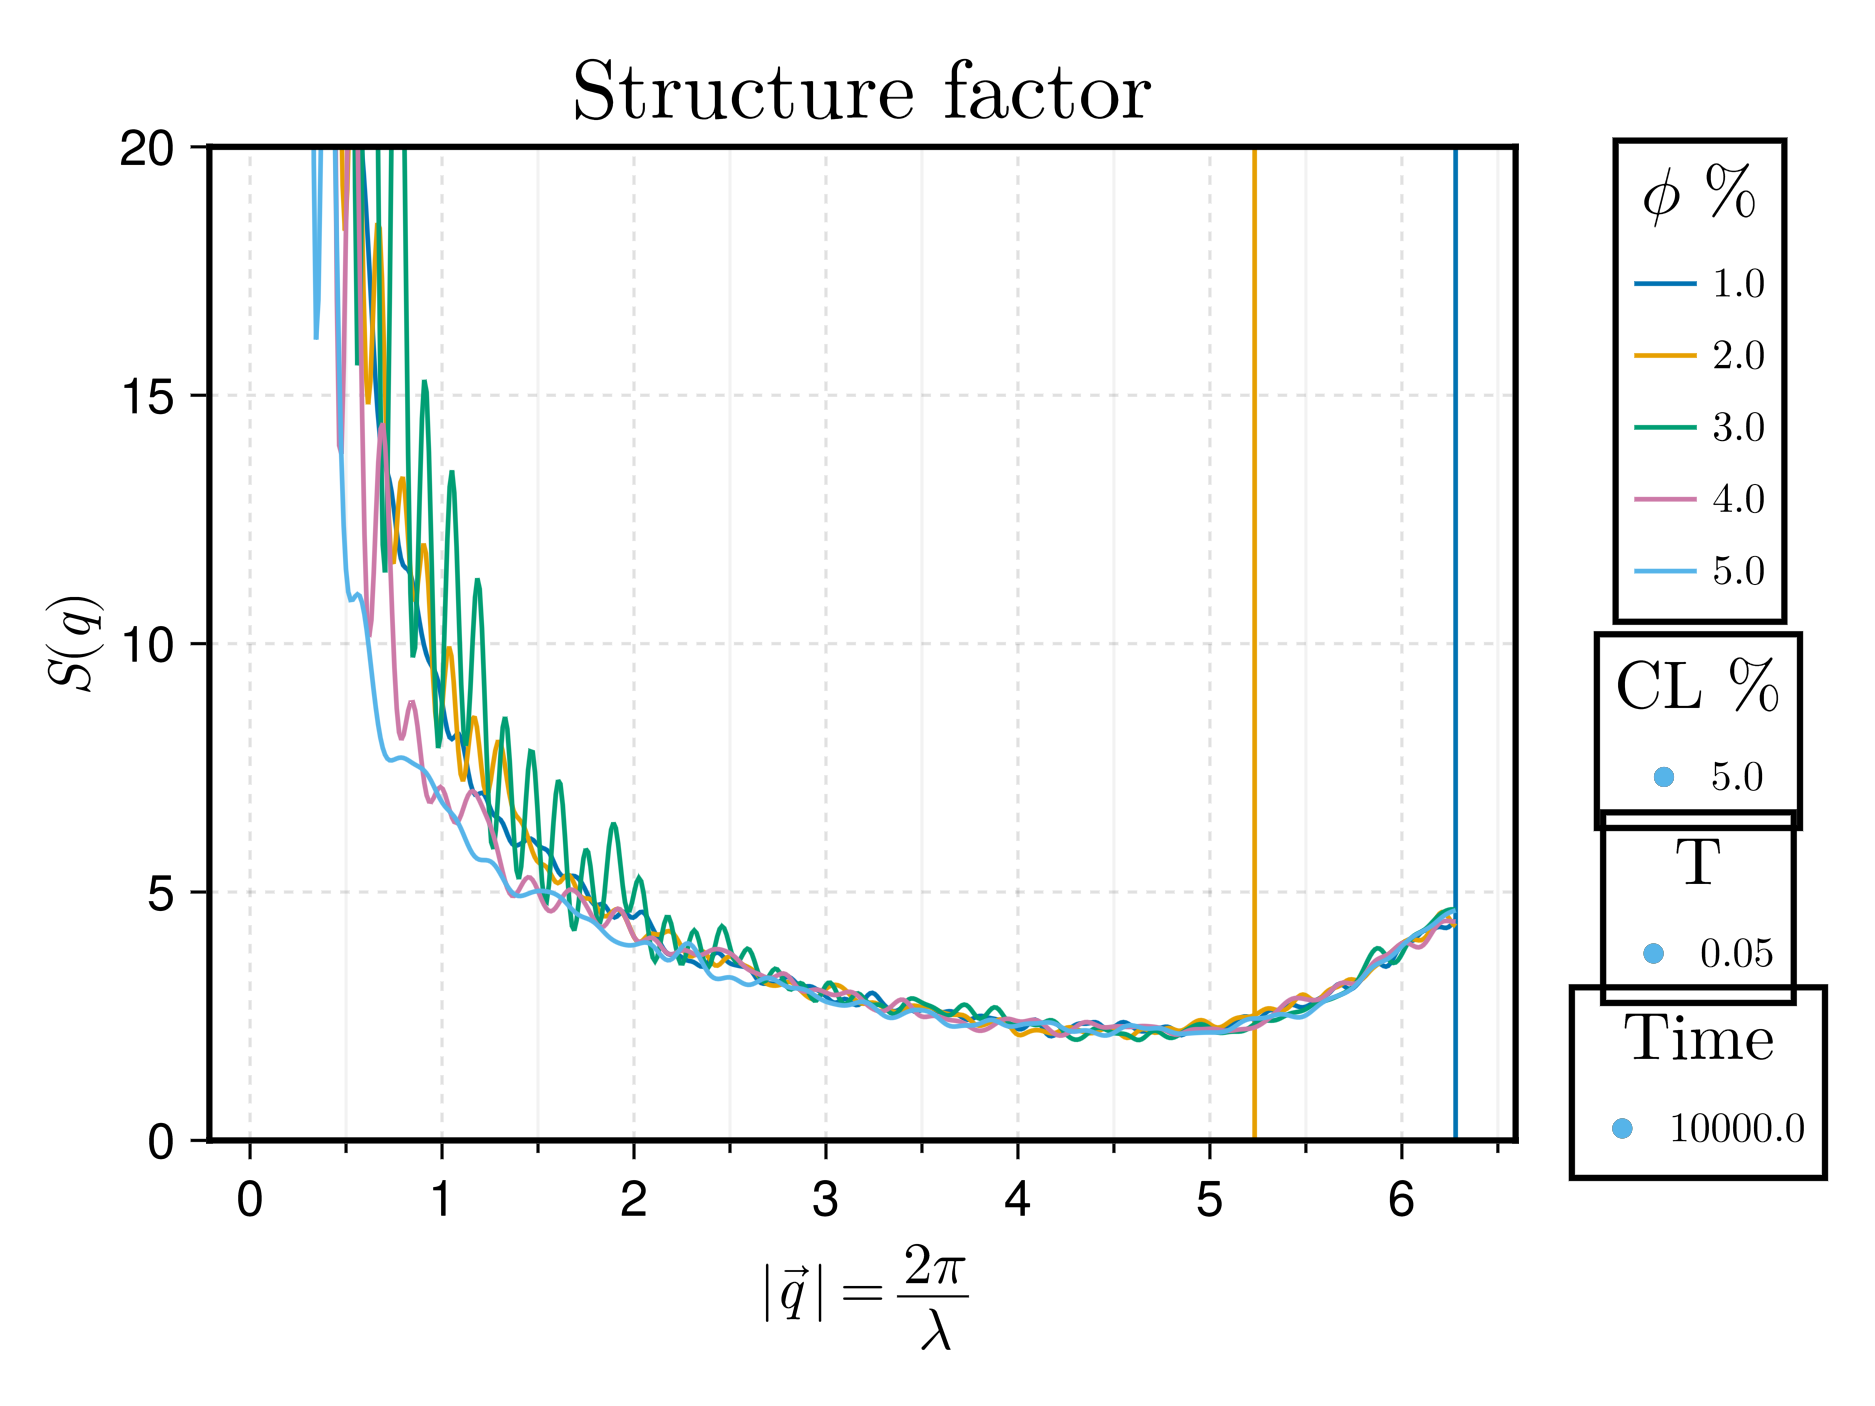
\includegraphics[width=0.9\textwidth]{../Figures/may4/fig_factorEstructuraCambios_tf_zoom.png}
    \caption{Comparación de los factores de estructura en el tiempo final de la simulación para distintas concentraciones. La línea vertical está ubicada en: \(2\pi,2\pi/1.2\).}
\end{figure}

Por el momento el número de direcciones es de \num{128}.
Por otro lado el número de magnitudes es de \num{512}.
No estoy seguro si aumentar el número de direcciones o realizar varios cálculos del factor de estructura y promediarlos.

No estoy seguro si aumentar el número de magnitudes.
Voy a intercambiar el número de magnitudes por el número de direcciones, a ver si cambia significativamente los resultados.

\newpage

\section{Explicación de cómo estoy calculando el factor de estructura}

De acuerdo con la expresión que \emph{pseudo-investigué} usando DeepSeek, estoy evaluando la siguiente función,
\begin{gather*}
    S(\vec{q}) = \frac{1}{N}\expval{A^{2} + B^{2}}
\end{gather*}
en donde,
\begin{gather*}
    A = \sum_{j=1}^{N}\cos\qty(\vec{q}\cdot\vec{r}_{j}),\quad
    B = \sum_{j=1}^{N}\sin\qty(\vec{q}\cdot\vec{r}_{j}).
\end{gather*}
Considerando que \(\vec{q} = \frac{2\pi}{\lambda}\hat{r}\) con \(\hat{r}\) siendo el vector de posición unitario en coordenadas esféricas\footnote{
    \begin{align*}
        r_1&=\cos\theta\sin\phi \\
        r_2&=\sin\theta\sin\phi \\
        r_3&=\cos\phi
    \end{align*}
}.
El producto punto se calcula de la siguiente manera,
\begin{align*}
    \vec{q}\cdot\vec{r}_{j}&=\frac{2\pi}{\lambda}\hat{r}\cdot\vec{r}_{j} \\
                           &=\frac{2\pi}{\lambda}\left(r_{1}^{j}r_{x} + r_{2}r^{j}_{y} + r_{3}r^{j}_{z} \right).
\end{align*}

Hay tres parámetros por definir, \(\lambda,\theta,\phi\).
Se pueden obtener $N_{\alpha}$ vectores unitarios para un solo valor de \(\lambda\).
Por otro lado el parámetro \(\lambda\) se restringue para el análisis de la red polimérica.
\(\lambda\in\qty[1,L]\), donde \(L\) es la lognitud de la caja.
Para obtener una curva lo suficientemente suave para el análisis se define \(N_{\lambda}=64=2^{6}\).


%Mi intución es que el producto punto no está evaluada.

\end{document}
